\pagestyle{empty}
\cleardoublepage
\pagestyle{fancy}
\chapter{Evolução de Modularidade em Diferentes Regimes de
Seleção}\label{cap4}

\section{Introdução}

Neste capitulo vamos utilizar o modelo com matriz $\mathbf{B}$ apresentado no
capítulo \ref{cap2} e parametrizado no capítulo \ref{cap3} para estudar
algumas possibilidades de trajetórias evolutivas responsáveis por moldar
o padrão de integração e modularidade de populações naturais. 
Novamente estamos interessados principalmente na evolução dos padrões de
covariação e surgimento de modularidade. 
Os parâmetros gerais usados nessas simulações são $p = 10$, $m = 50$,
$\mu/\mu_B = 5$, $Ne = 5.000$. 

\section{Estabelecimento de equilíbrio}

Afim de minimizar ao máximo a influência de estados iniciais das
populações, todas as simulações nesse capítulo são baseadas na mesma
população inicial, que por sua vez passou por 10.000 gerações de deriva
pura, sem seleção de qualquer tipo, seguidos de 10.000 gerações de
seleção estabilizadora correlacionada com matriz $\omega$ com dois
módulos, como na equação \ref{matw}. 
No primeiro período, de deriva, garantimos que o estado inicial é
totalmente perdido por ação de mutação e deriva. 
Depois, durante a seleção estabilizadora, garantimos que a população
esteja em equilíbrio seleção-mutação-deriva, mas ainda com variação
suficiente para responder à seleção direcional. 
Padronizando as populações iniciais podemos isolar de forma mais
sistemática efeitos de diferentes regimes de seleção. 
Na figura \ref{varBurnin} observamos a evolução das variâncias
fenotípicas, variâncias genéticas dos valores aditivos e da
herdabilidade para todos os 10 caracteres da população. 
Notamos que inicialmente as variâncias crescem rapidamente, pois sem
seleção a mutação introduz nova variação a cada geração que só pode ser
removida por deriva. 
Como a população é bastante grande ($Ne = 5.000$), a remoção é lenta e o
equilíbrio mutação-deriva se dá num valor de variância muito alto
(comparado com a variância ambiental ou variância do erro $e$, veja
capítulo \ref{cap2}, equação \ref{matrizB}). 
Nas mesmas figuras, após 10.000 gerações de deriva, foi imposto um regime de
seleção estabilizadora correlacionada. 
Imediatamente as variâncias genéticas e fenotípicas caem bruscamente
para os valores de equilíbrio seleção-mutação-deriva, e o sistema se
estabiliza nesses valores. 
Podemos ver no painel \ref{Corr} o efeito sobre as correlações,
que também diminuem com a remoção seletiva da variabilidade dessa
população. 
A seleção estabilizadora é mantida por 10.000 gerações. 


\begin{figure}[htbp]
   \centering
   \subfloat [Variâncias Fenotípicas]{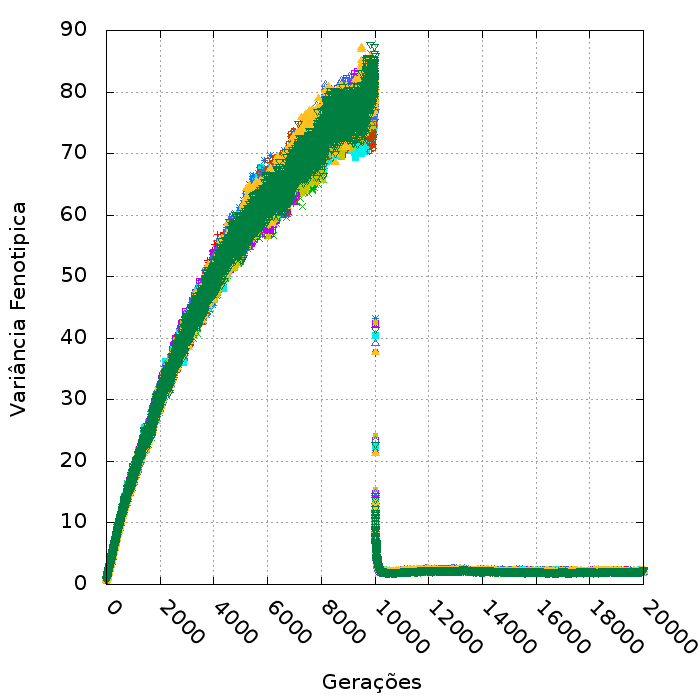
\includegraphics[width=70mm, height=70mm]{figuras/varBurninP.png}}\vspace{11pt}
   \subfloat [Variâncias Genéticas]{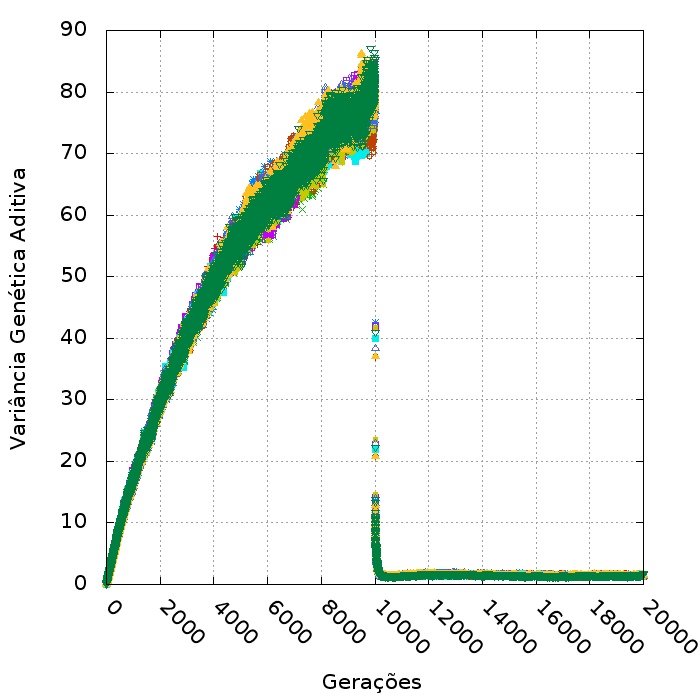
\includegraphics[width=70mm, height=70mm]{figuras/varBurninG.png}}\\ 
   \vspace{-18pt}
   \subfloat [Herdabilidade]{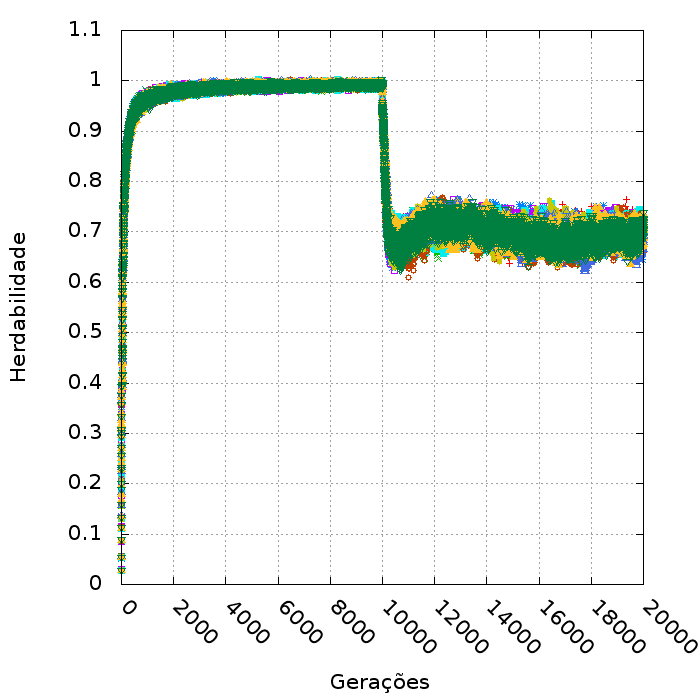
\includegraphics[width=70mm, height=70mm]{figuras/varBurninH.png}}\vspace{11pt} 
   \subfloat [Correlações]{\label{Corr}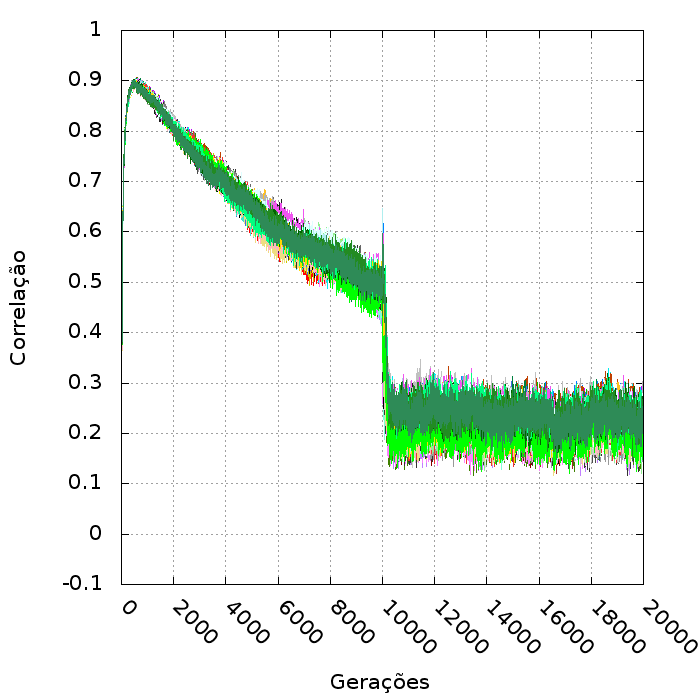
\includegraphics[width=70mm, height=70mm]{figuras/varBurninCorr.png}}\\
   \caption{Evolução de variâncias fenotípicas e genéticas,
   herdabilidades e correlações para uma população passando por 10.000
gerações de deriva, seguidas de 10.000 gerações de seleção
estabilizadora correlacionada ($Ne = 5.000$, $m/p=5$, $\mu/\mu_B=5$).}
   \label{varBurnin}
\end{figure}


\section{Seleção Direcional}

Tomados os cuidados com a inicialização da população, iniciamos o
regime de seleção direcional com intensidade variáveis, como na seção
\ref{cap3:DirecB}. 
Novamente nossa seleção é medida por mudanças no pico adaptativo, com
$\Delta_S$ de $0.01$ até $0.2$. 
Todas os caracteres sofrem seleção direcional simultânea correlacionada,
de aumento nos $5$ primeiros e diminuição nos $5$ últimos, de forma
concordante com estrutura modular da seleção estabilizadora
correlacionada.
Calculamos os valores de $|\beta_i|$, afim de comparar nossa
intensidade de seleção com aquela medida em populações naturais.
Os resultados estão na tabela \ref{tab:betasMFM}.
Valores de AVG-Ratio e modularidade $L$ para essas corridas podem ser
vistos na figura \ref{MFMStats}. 
Incluímos também, por clareza, as últimas gerações de seleção
estabilizadora, a seleção direcional começa a atuar a partir da geração
20.000. 

\begin{table}[htbp]
    \centering
    \caption{Intensidades de seleção, representadas pelo diferencial de
        seleção por caráter e pelo valor do gradiente de seleção por caráter
    $|\beta_i|$}
    \label{tab:betasMFM}
    \vspace{1em}
    \begin{tabular}{c|c|c|c|c|c}
        \toprule
        $\Delta_S$ & 0.01 & 0.02 & 0.03 & 0.04 & 0.05 \\
        \hline
        $|\beta_i|$ médio & 0.0016 & 0.0032 & 0.0048 & 0.0062 & 0.0076 \\
         $|\beta_i|$ total & 1.466 & 2.908 & 4.325 & 5.588 & 6.872 \\
        \midrule
        \midrule
        $\Delta_S$ & 0.06 & 0.07 & 0.08 & 0.09 & 0.10 \\
        \hline
        $|\beta_i|$ médio & 0.0088 & 0.0103 & 0.0115 & 0.0128 & 0.0143 \\        
         $|\beta_i|$ total & 7.975 & 9.290 & 10.398 & 11.583 & 12.913 \\
        \midrule
        \midrule
        $\Delta_S$ & 0.11  & 0.12  & 0.13  & 0.14  & 0.15 \\ 
        \hline
        $|\beta_i|$ médio & 0.0152 & 0.0165 & 0.0175 & 0.0186 & 0.0200 \\    
         $|\beta_i|$ total & 13.726 & 14.920 & 15.759 & 16.746 & 18.054 \\
        \midrule
        \midrule
        $\Delta_S$ & 0.16  & 0.17  & 0.18  & 0.19  & 0.20  \\ 
        \hline
        $|\beta_i|$ médio & 0.0209 & 0.0224 & 0.0238 & 0.0242 & 0.0254 \\
         $|\beta_i|$ total & 18.899 &  20.201 & 21.490 & 21.821 & 22.913  \\
        \bottomrule
    \end{tabular}
\end{table}

Nessa condições, o sistema se modulariza rapidamente a partir de uma dada
intensidade de seleção.
O aumento tanto da modularidade $L$ quanto do AVG-Ratio, indica presença
de modularidade variacional na estrutura de covariação da população
simulada.
A concordância desses duas estatísticas nos leva a crer que os módulos
presentes na superfície de seleção estão realmente se manifestando na
estrutura de covariação da população.
Podemos ainda dissecar o efeito da seleção direcional nas correlações
dentro e entre módulos, olhando para a evolução de cada uma
separadamente. 
Na figura \ref{AVGEntreIntra} podemos ver essa separação para diferentes
valores de $\Delta_S$. 
O padrão de aumento das correlações dentro módulos é esperado. 
Além disso, observamos uma concomitante diminuição das correlações entre
módulos. 
Novamente, isso é característico de uma estrutura variacional modular,
com duas classes de correlação correspondendo a relação de caracteres
dentro e entre módulos.
Como cada módulo responde a forças seletivas antagônicas, a correlação
entre eles tente a diminuir, permitindo que os caracteres dentro de cada
módulo evoluam independentemente dos outros módulos. 
Isso é coerente com simulações em sistemas simples feitas por
\cite{Pavlicev2010} utilizando a equação
de reposta a seleção de \cite{Lande1979} e a existência de rQTLs
\citep{Pavlicev2008a}. 
Neste artigo os autores descrevem como seleção direcional pode favorecer
ativamente a criação de linhas de menor resistência evolutiva
\citep[direções do espaço morfológico ricas em
variação, veja][]{Schluter1996},  alinhadas com a seleção. 
Reorganização de estrutura variacional relacionada a eventos de seleção
prolongada também já foram descritos na literatura \citep{Berg1960,
Young2005, Young2010}. 
Nossos resultados mostram que isso pode acontecer em sistemas
bastante complexos, via seleção indireta nos padrões de
covariação, gerando variação nas direções privilegiadas pela seleção
direcional e aumentando a evolvabilidade das populações. 
Evolvabilidade é definida como a projeção da resposta evolutiva na
direção privilegiada pela seleção natural \citep{Hansen2008}.
Esse valor é controlado por dois fatores: a intensidade da pressão
seletiva, seleção direcional mais intensa provoca mudanças maiores; e
pela quantidade de variação disponível na população na direção da
seleção direcional, caso a população não possua variação herdável na
direção da seleção, não existe resposta evolutiva.
O alinhamento da estrutura de covariação da população com o vetor de
seleção basicamente representa o aumento de variação fenotípica da
população na direção da seleção.
Dessa forma, esse tipo de plasticidade na estrutura de covariação pode
ser muito vantajosa, permitindo com que populações sofrendo seleção
direcional aumentem sua variabilidade na direção da seleção, aumentando
sua resposta adaptativa.

\begin{figure}[htbp]
   \centering
   \subfloat [$\Delta_S = 0.01$]{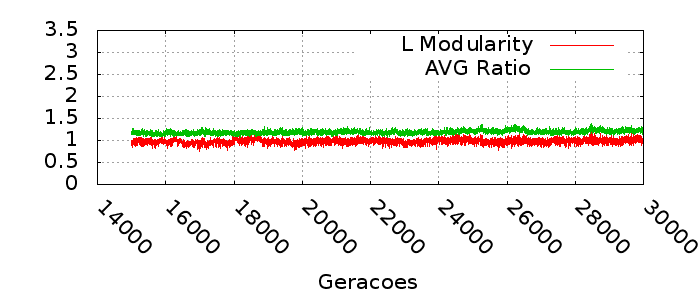
\includegraphics[width=70mm, height=30mm]{figuras/MFMStats10.png}}\vspace{11pt}
   \subfloat [$\Delta_S = 0.03$]{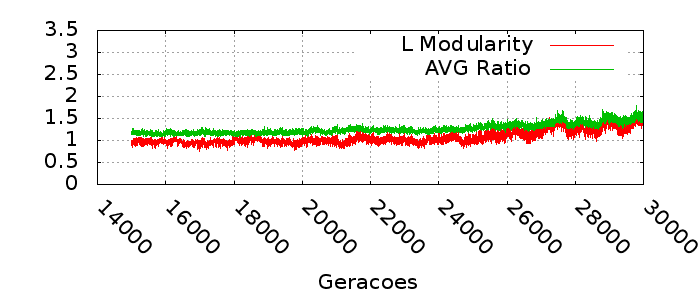
\includegraphics[width=70mm, height=30mm]{figuras/MFMStats30.png}}\\ 
   \vspace{-18pt}
   \subfloat [$\Delta_S = 0.05$]{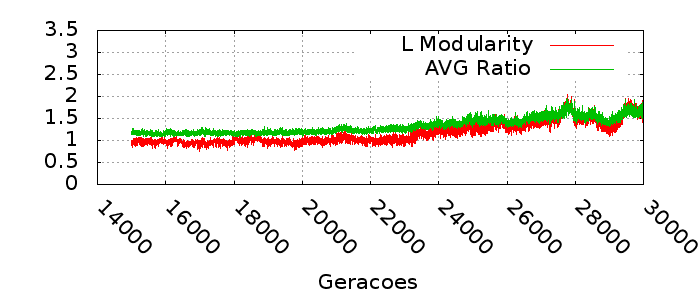
\includegraphics[width=70mm, height=30mm]{figuras/MFMStats50.png}}\vspace{11pt} 
   \subfloat [$\Delta_S = 0.07$]{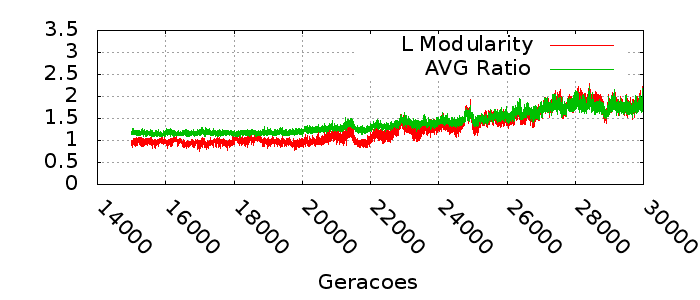
\includegraphics[width=70mm, height=30mm]{figuras/MFMStats70.png}}\\
   \vspace{-18pt}
   \subfloat [$\Delta_S = 0.09$]{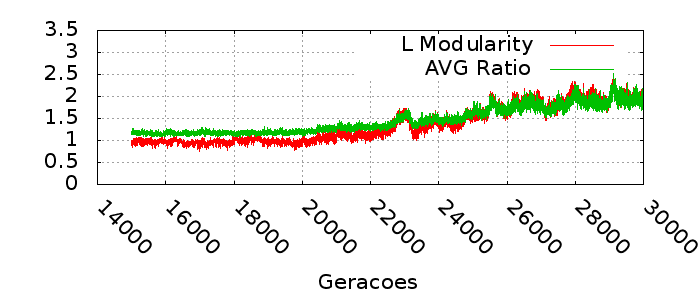
\includegraphics[width=70mm, height=30mm]{figuras/MFMStats90.png}}\vspace{11pt}
   \subfloat [$\Delta_S = 0.11$]{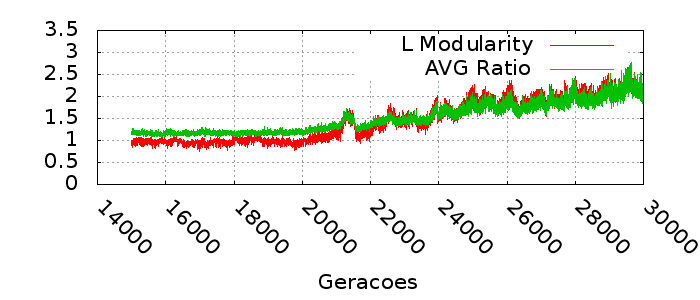
\includegraphics[width=70mm, height=30mm]{figuras/MFMStats110.png}}\\
   \vspace{-18pt}
   \subfloat [$\Delta_S = 0.13$]{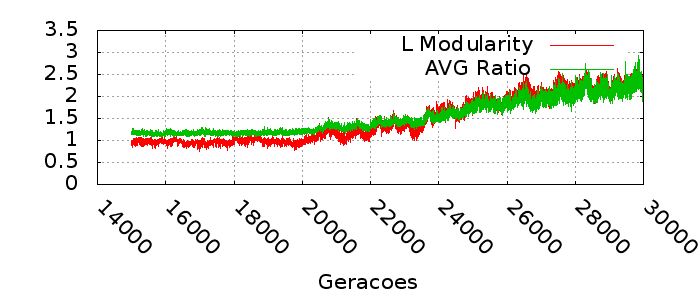
\includegraphics[width=70mm, height=30mm]{figuras/MFMStats130.png}}\vspace{11pt}
   \subfloat [$\Delta_S = 0.15$]{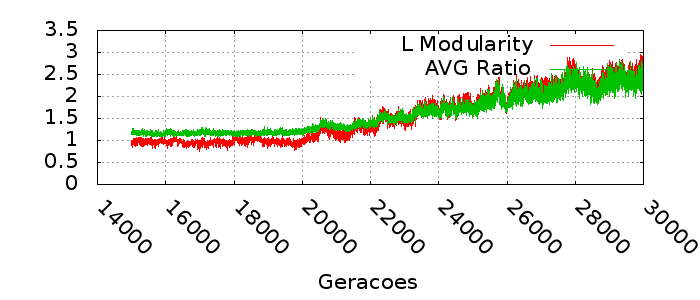
\includegraphics[width=70mm, height=30mm]{figuras/MFMStats150.png}}\\
   \vspace{-18pt}
   \subfloat [$\Delta_S = 0.17$]{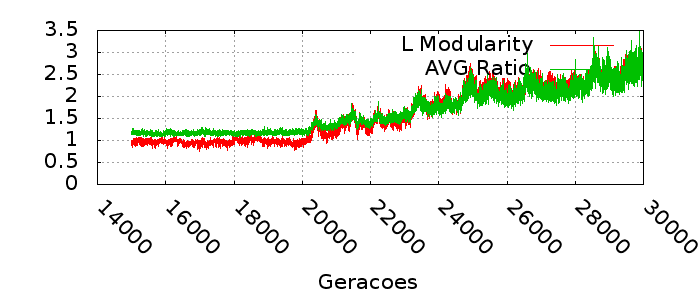
\includegraphics[width=70mm, height=30mm]{figuras/MFMStats170.png}}\vspace{11pt}
   \subfloat [$\Delta_S = 0.19$]{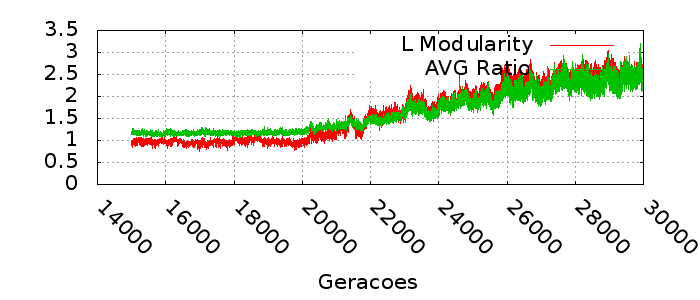
\includegraphics[width=70mm, height=30mm]{figuras/MFMStats190.png}}\\
   \caption{ AVG-Ratio e modularidade $L$ para corridas com
      $\mu/\mu_B = 5$, $Ne = 5.000$, $m/p=5$, sofrendo seleção
      estabilizadora correlacionada com 2 módulos e seleção direcional com
   diferentes valores de $\Delta_S$. Seleção direcional a partir da
   geração $20.000$.}
   \label{MFMStats}
\end{figure}

\begin{figure}[htbp]
   \centering
   \subfloat [$\Delta_S = 0.01$]{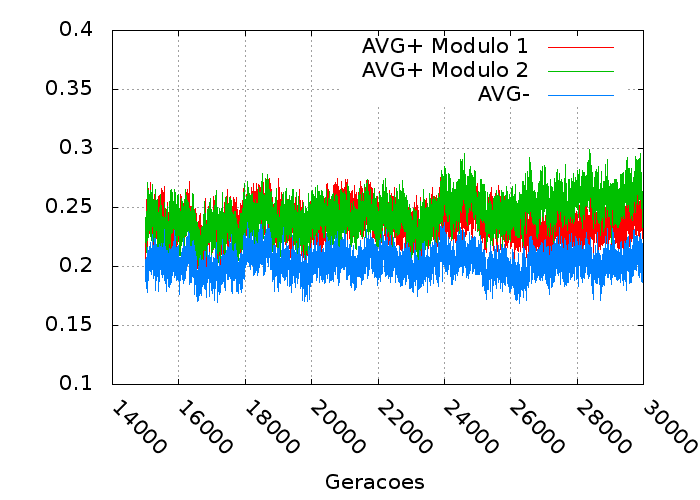
\includegraphics[width=70mm, height=50mm]{figuras/AVGPlusMinus10.png}}\vspace{11pt}
   \subfloat [$\Delta_S = 0.03$]{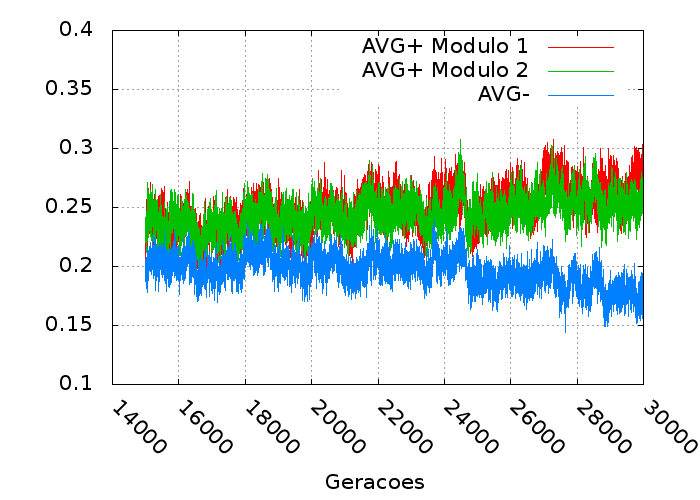
\includegraphics[width=70mm, height=50mm]{figuras/AVGPlusMinus30.png}}\\ 
   \vspace{-18pt}
   \subfloat [$\Delta_S = 0.09$]{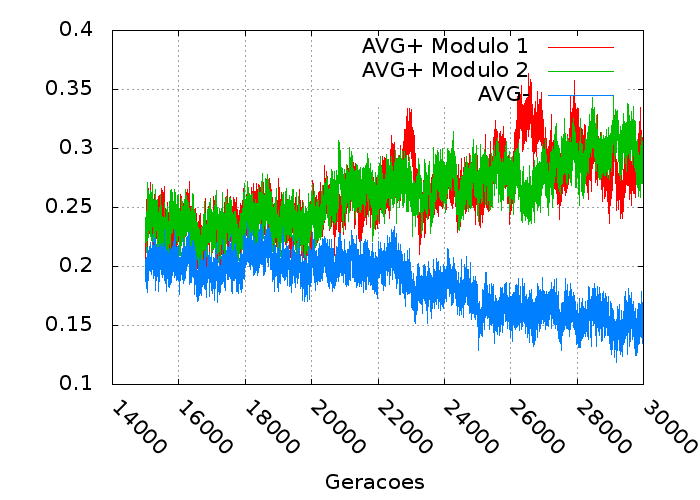
\includegraphics[width=70mm, height=50mm]{figuras/AVGPlusMinus90.png}}\vspace{11pt}
   \subfloat [$\Delta_S = 0.11$]{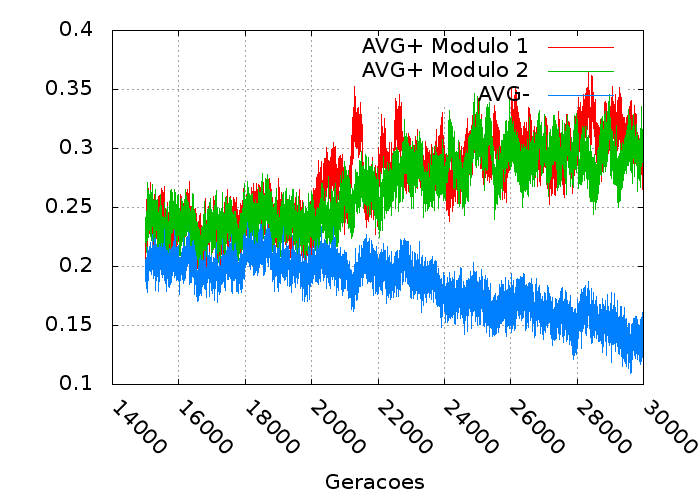
\includegraphics[width=70mm, height=50mm]{figuras/AVGPlusMinus110.png}}\\
   \vspace{-18pt}
   \subfloat [$\Delta_S = 0.18$]{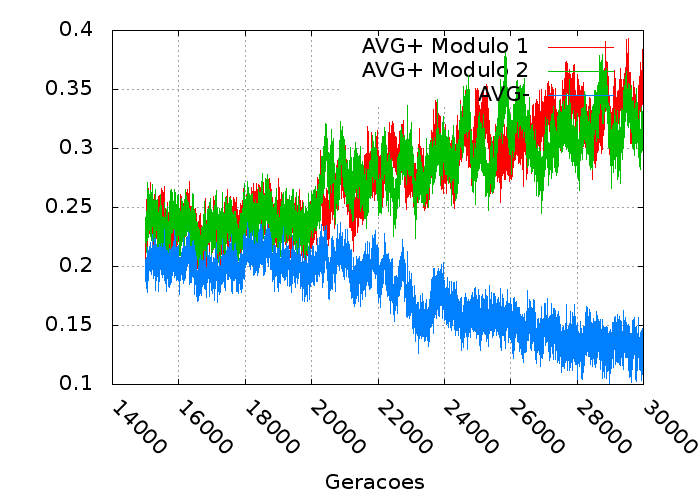
\includegraphics[width=70mm, height=50mm]{figuras/AVGPlusMinus180.png}}\vspace{11pt}
   \subfloat [$\Delta_S = 0.20$]{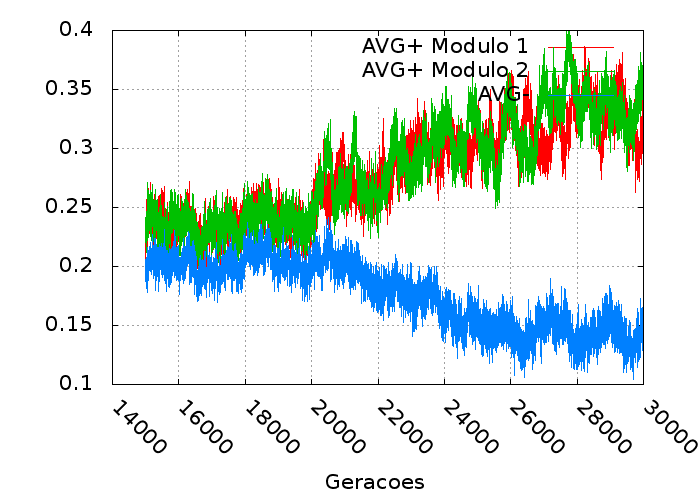
\includegraphics[width=70mm, height=50mm]{figuras/AVGPlusMinus200.png}}\\
   \caption{ Evolução da média das correlações dentro de cada módulo
      e entre módulos de uma população sofrendo seleção estabilizadora
      correlacionada com 2 módulos e seleção direcional com diferentes
   valores de $\Delta_S$. $\mu/\mu_B = 5$, $Ne = 5.000$, $m/p=5$. Seleção
   direcional a partir da geração $20.000$.}
   \label{AVGEntreIntra}
\end{figure}

\centerline { $ * \quad * \quad * $ }

Nossos valores de seleção direcional, apesar de promoverem
diferenciações extremas ao longo de milhares de gerações, são
relativamente baixos se comparados com estimativas em populações
naturais.
Nesse seção, o valor mais alto de diferencial de seleção direcional
($\Delta_S = 0.2$), levando em conta a
estrutura de covariação emergente da população, resultou em um gradiente de
seleção médio de apenas $|\beta_i| = 0.0254$.
Com esse gradiente baixo, apenas $15\%$ de um gradiente típico em
sistemas morfológicos e apenas $2\%$ de um gradiente extremo
\citep{Kingsolver2001}, nós observamos modularidade aparecendo de forma
inequívoca em apenas alguns milhares de gerações, dependendo da força da
seleção direcional aplicada (figuras \ref{MFMStats} e
\ref{AVGEntreIntra}).
Partindo das mesmas populações iniciais, já em equilíbrio
seleção-mutação-deriva, decidimos então testar gradientes de seleção
mais extremos, com corridas durando apenas $1.000$ gerações.
Essas populações foram submetidas a forças de seleção $10\times$ maiores que
as anteriores, com $\Delta_S$ variando de $0.1$ até $2.0$. 
Dessa forma, a quantidade de modificação fenotípica total permaneceu
constante, mas os gradientes de seleção foram aumentados sensivelmente.
A relação dos $|\beta_i|$ calculados para uma corrida aparece na tabela
\ref{tab:betasSS}.
Os $|\beta_i|$ totais são semelhantes aos da tabela \ref{tab:betasMFM},
porém os $|\beta_i|$ médios são cerca de $10\times$ maiores, como esperado.
Podemos comparar a evolução das correlações para as corridas de $10.000$
gerações de seleção com as de $1.000$ gerações.
Vemos esses dados na figura \ref{MFMxSS}, para alguns valores de
$\Delta_S$.
Ao final das corridas, vemos valores bastante semelhantes para os
valores de correlações médias dentro e entre módulos.
Isso sugere que o tempo em gerações para o sistema assumir um nível
determinado de modularidade depende linearmente da força de seleção
aplicada.

Podemos quantificar o tempo de convergência da estrutura variacional da
população para a estrutura de covariação da seleção direcional medindo
diretamente a correlação da matriz de correlação da população com a
matriz de correlação da superfície de seleção.
Vemos esses resultados na figura \ref{CorrMat}, onde são mostrados a
correlação entre a matriz de correlação da população a cada geração com
a matriz $\omega$ da superfície de seleção, para os
extremos de força de seleção direcional nas corridas curtas, de $1.000$
gerações, e longas, de $10.000$, além de todo o periodo de inicialização
descrito anteriormente, que serviu de estado inicial para ambas as
corridas seletivas.
Aqui vemos uma diferença entre os dois tipos  de simulação.
Para as corridas longas, sobre seleção fraca ($\Delta_S = 0.01$) a
correlação entre as matrizes não aumenta, enquanto para seleção forte
($\Delta_S = 0.2$), após cerca de $4.000$ gerações a correlação chega
num patamar estável mais alto.
Nas corridas curtas isso não acontece, e a semelhança da matriz não se
estabiliza após um período correspondente, só se tornando
consistentemente mais alto que na corrida com seleção mais baixa após
cerca de $750$ gerações.
Com isso vemos que a dinâmica da resposta à seleção direcional não é
totalmente linear, e existem complicações associadas à
interação entre a quantidade de variação introduzida na população por
mutação e a variação removida pela seleção natural.
Quando aumentamos a intensidade da seleção direcional, mais variação é
removida a cada geração pela seleção, e o número de indivíduos que
compõem a próxima geração diminui, pelo aumento na variância dos valores
de aptidão causado pela distância maior entre o pico adaptativo e a
média da população.
Uma consequência desse ``gargalo seletivo'' é o aumento da deriva genética,
que implica numa variação maior da estrutura de covariação.
Todos esses fatores contribuem para que a população demore mais para se
estabilizar na estrutura de covariação privilegiada pela seleção, e a
correlação entre a matriz de correlação da população e da superfície de
seleção acaba flutuando muito e não aumentando tanto quanto no caso de
seleção mais fraca e continuada.

\begin{table}[htbp]
    \centering
    \caption{Intensidades de seleção, representadas pelo diferencial de
        seleção por caráter e pelo valor do gradiente de seleção por
        caráter $|\beta_i|$ para as simulações com $1.000$ gerações de
        seleção direcional correlacionada.}
    \label{tab:betasSS}
    \vspace{1em}
    \begin{tabular}{c|c|c|c|c|c}
        \toprule
        $\Delta_S$ & 0.1 & 0.2 & 0.3 & 0.4 & 0.5 \\
        \hline
        $|\beta_i|$ médio & 0.014 & 0.025 & 0.036 & 0.048 & 0.057 \\
         $|\beta_i|$ total & 1.431 & 2.564 & 3.640 & 4.824 & 5.786 \\ 
        \midrule
        \midrule
        $\Delta_S$ & 0.6 & 0.7 & 0.8 & 0.9 & 1.0 \\
        \hline
        $|\beta_i|$ médio & 0.066 & 0.077 & 0.087 & 0.098 & 0.104 \\
         $|\beta_i|$ total & 6.629 & 7.782 & 8.792 & 9.898 & 10.454 \\ 
        \midrule
        \midrule
        $\Delta_S$ & 1.1  & 1.2  & 1.3  & 1.4  & 1.5 \\ 
        \hline
        $|\beta_i|$ médio & 0.113 & 0.129 & 0.138 & 0.157 & 0.154 \\
         $|\beta_i|$ total & 11.348 & 12.937 & 13.875 & 15.733 & 15.499 \\ 
        \midrule
        \midrule
        $\Delta_S$ & 1.6  & 1.7  & 1.8  & 1.9  & 2.0 \\ 
        \hline
        $|\beta_i|$ médio & 0.163 & 0.177 & 0.184 & 0.207 & 0.207 \\
         $|\beta_i|$ total & 16.305 & 17.702 & 18.441 & 20.762 & 20.775 \\
        \bottomrule
    \end{tabular}
\end{table}

\begin{figure}[htbp]
   \centering
   \subfloat [$\Delta_S = 0.01$]{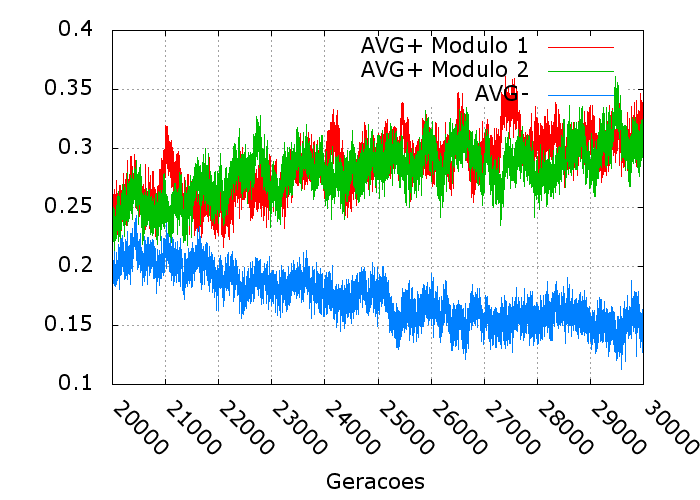
\includegraphics[width=70mm, height=50mm]{figuras/AVGPM10.png}}\vspace{11pt}
   \subfloat [$\Delta_S = 0.1$]{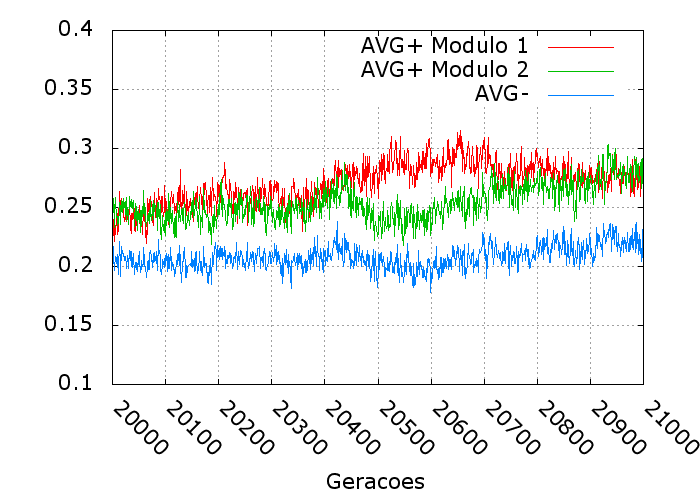
\includegraphics[width=70mm, height=50mm]{figuras/AVGPMShortSel10.png}}\\ 
   \vspace{-18pt}
   \subfloat [$\Delta_S = 0.11$]{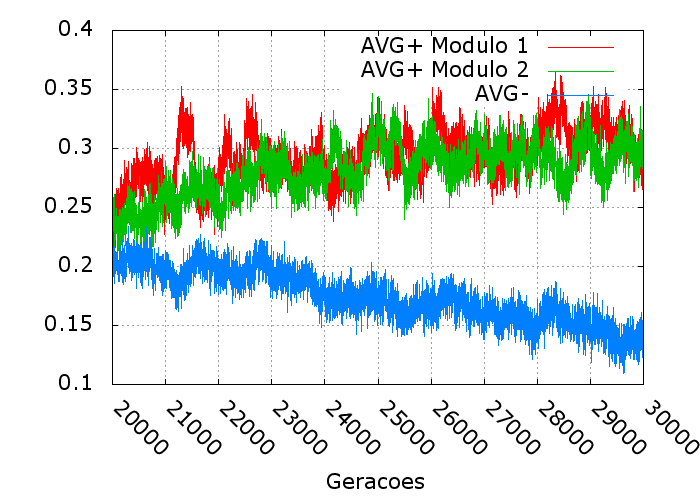
\includegraphics[width=70mm, height=50mm]{figuras/AVGPM110.png}}\vspace{11pt}
   \subfloat [$\Delta_S = 1.1$]{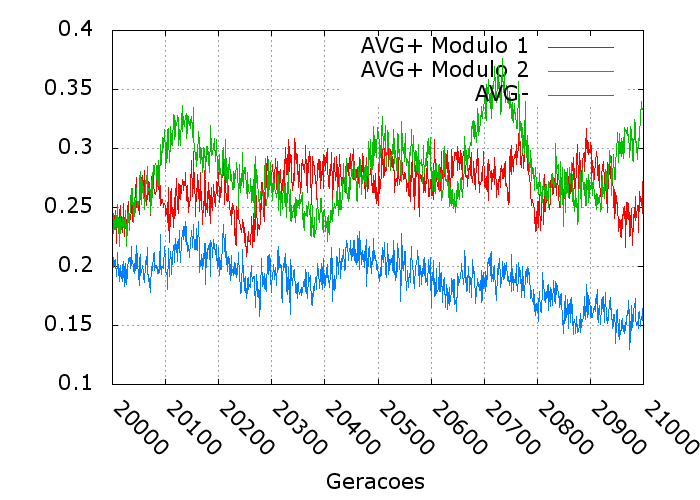
\includegraphics[width=70mm, height=50mm]{figuras/AVGPMShortSel110.png}}\\
   \vspace{-18pt}
   \subfloat [$\Delta_S = 0.2$]{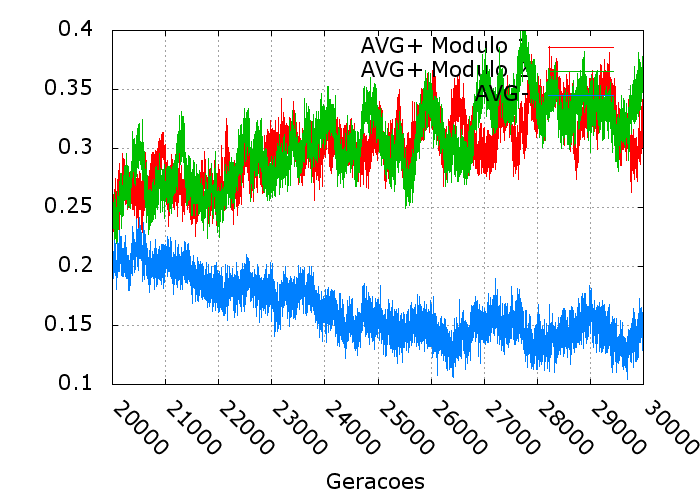
\includegraphics[width=70mm, height=50mm]{figuras/AVGPM200.png}}\vspace{11pt}
   \subfloat [$\Delta_S = 2.0$]{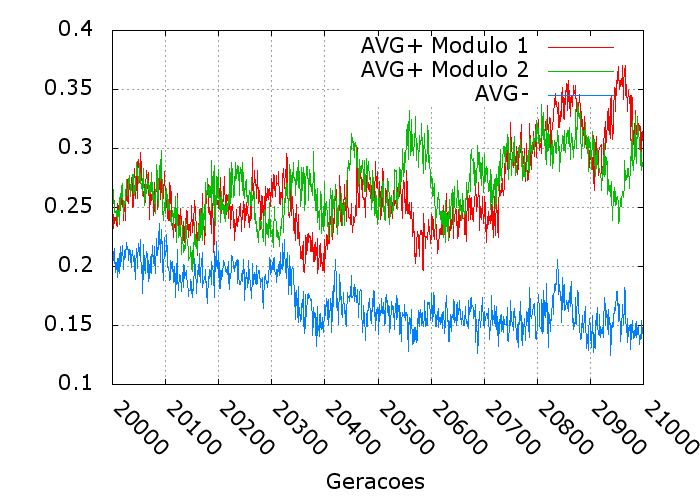
\includegraphics[width=70mm, height=50mm]{figuras/AVGPMShortSel200.png}}\\
   \caption{ Evolução da média das correlações dentro de cada módulo
      e entre módulos de uma população sofrendo seleção estabilizadora
      correlacionada com 2 módulos e seleção direcional com diferentes
   valores de $\Delta_S$. $\mu/\mu_B = 5$, $Ne = 5.000$, $m/p=5$. 
   Todas as populações partem da mesma população inicial, e cada linha
   tem o mesmo $|\beta_i|$ total ao final da corrida. São mostradas apenas
   as gerações de seleção direcional.}
   \label{MFMxSS}
\end{figure}

\begin{figure}[htbp]
   \centering
   \subfloat [Estabelecimento do equilíbrio inicial]{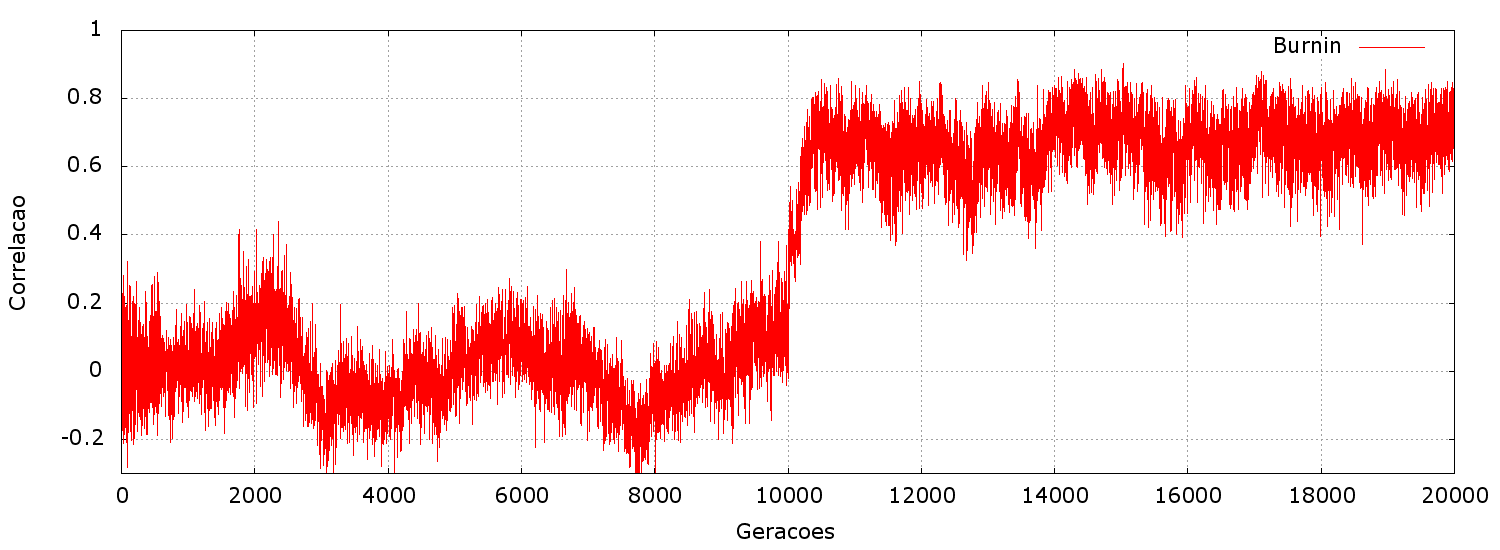
\includegraphics[width=140mm, height=50mm]{figuras/CorMatBurnin.png}}\\ 
   \subfloat [$\Delta_S = (0.01, 0.2)$, $10.000$ gerações]{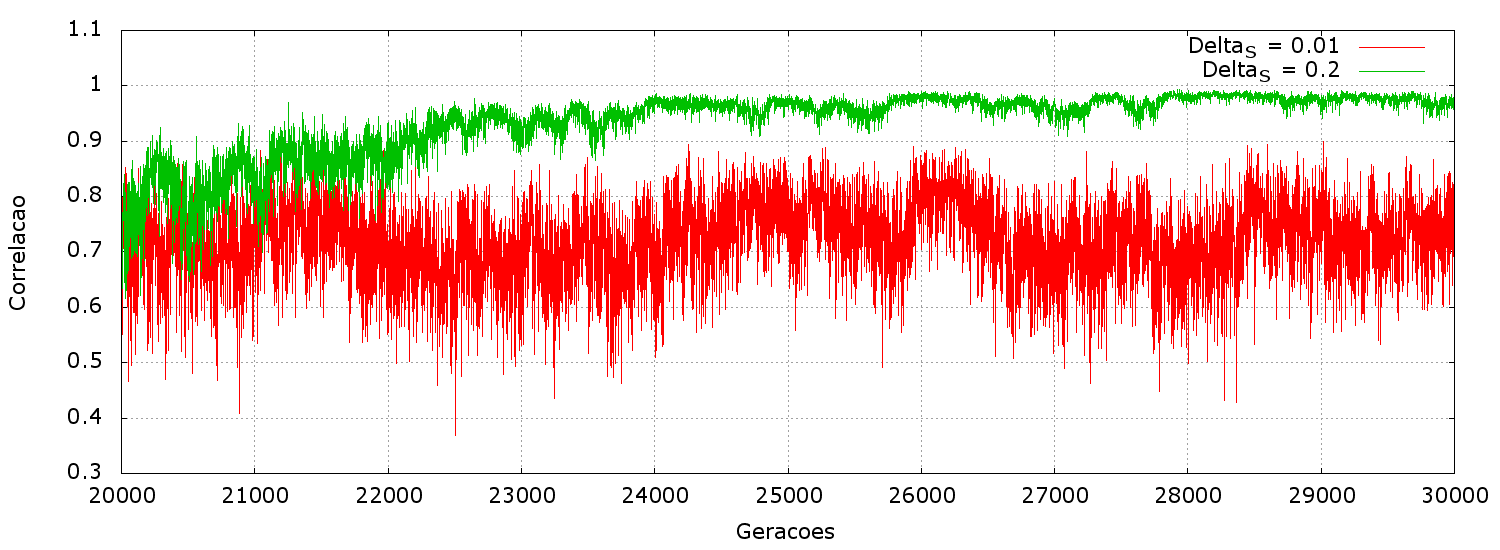
\includegraphics[width=140mm, height=50mm]{figuras/CorMatMFM.png}}\\ 
   \subfloat [$\Delta_S = (0.1, 2.0)$, $1.000$ gerações]{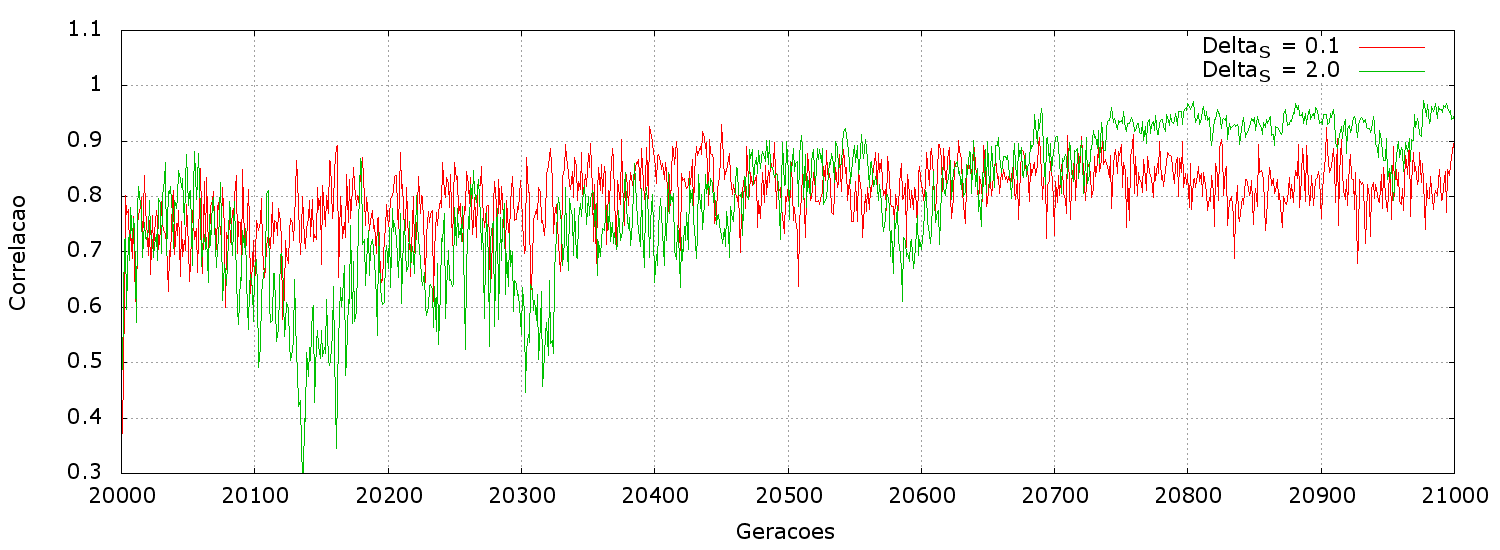
\includegraphics[width=140mm, height=50mm]{figuras/CorMatSS.png}}\vspace{11pt}
   \caption{ Evolução da correlação entre a matriz de correlação da
       população a cada geração com a matriz de correlação da superfície
       de seleção $\omega$, para corridas de diferentes números de
       gerações e intensidades de seleção direcional divergente entre
   módulos. O painel (a) mostra a evolução da correlação antes da
   seleção direcional, com $10000$ gerações de deriva e $10.000$
   gerações de seleção estabilizadora correlacionada. $\mu/\mu_B = 5$, $Ne = 5.000$, $m/p=5$}
   \label{CorrMat}
\end{figure}

\section{Seleção direcional ``corredor''}

Seleção direcional parece então ser fundamental para o surgimento de
módulos variacionais nas nossas simulações. 
Porém, a situação onde todos os caracteres de um complexo morfológico estão
sobre seleção simultânea divergente não parece ser uma regra na
natureza, ou pelo menos é difícil acreditar que todas as instâncias de
modularidade variacional sejam devido a eventos de seleção direcional
divergente em todos os caracteres dos módulos envolvidos simultaneamente. 
Seria a seleção natural sobre apenas um conjuntos de caracteres capaz de
gerar modularidade do mesmo tipo?
Para responder essa pergunta nós começamos com a mesma população
inicial, mas agora apenas um dos módulos era sujeito a seleção
direcional, com o outro conjunto de caracteres mantido constante pela
seleção estabilizadora. 
Novamente a matriz de seleção da superfície adaptativa era não diagonal,
impondo seleção estabilizadora correlacionada na população.
Esse cenário evolutivo é conhecido como evolução ``corredor'', pois uma
parte dos caracteres se altera por ação da seleção direcional (ao
longo do corredor) enquanto o outro conjunto está restrito por ação de
seleção estabilizadora (entre as paredes do corredor). 

Na figura \ref{CoAVG} vemos a evolução das correlações dentro e entre
módulos para esse cenário evolutivo. 
Primeiro destacamos que novamente as correlações entre módulo decaem, de
forma semelhante ao caso de seleção direcional divergente nos dois
módulos. 
O módulo sobre seleção direcional também se comporta de forma semelhante
ao caso anterior, com correlações aumentando ao longo da simulação. 
Porém, nessas simulações são geradas 3 classes de correlação. 
As correlações dentro do módulo sofrendo apenas seleção estabilizadora
também aumentam, ainda que de forma menos acentuada que as do módulo que
sofre seleção direcional. 
Em alguns casos as correlações dentro do módulo com seleção
estabilizadora chegam ao mesmo nível médio que o módulo sofrendo seleção
direcional, como no painel \ref{CoAVG:Igual}. 
À medida que a seleção direcional aumenta, a distinção entre os dois
módulos se torna mais acentuada. 
Esses resultados apontam para um mecanismo plausível de formação de
módulos variacionais em populações naturais. 
Como a seleção em um grupo de caracteres é suficiente para gerar
modularidade na estrutura de covariação completa na população, incluindo
caracteres não diretamente envolvidos na seleção direcional, eventos
subsequentes de seleção direcional em grupos distintos de caracteres
morfológicos podem gerar o padrão intrincado de módulos que observamos na
natureza, sem para isso ser necessária a atuação de seleção direcional
divergente simultânea sobre todos os módulos. 

\begin{figure}[p]
   \centering
   \subfloat [$\Delta_S = 0.01$]{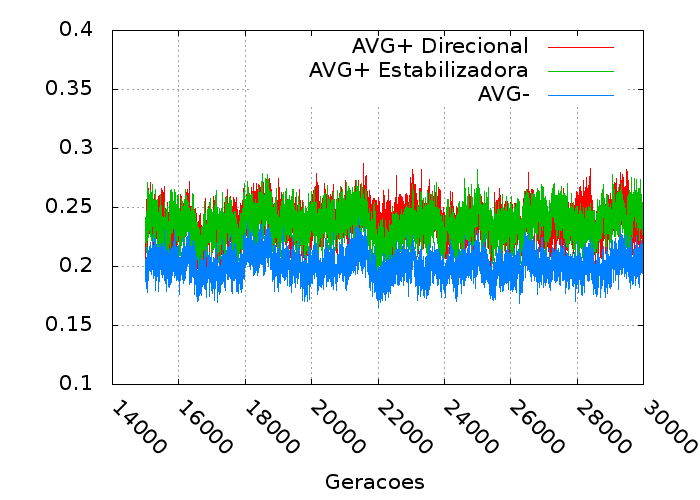
\includegraphics[width=70mm, height=50mm]{figuras/CoAVGPM10.png}}\vspace{11pt}
   \subfloat [$\Delta_S = 0.03$]{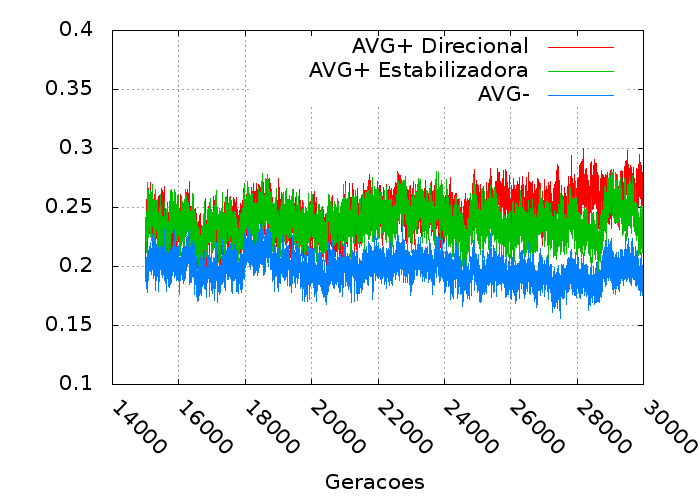
\includegraphics[width=70mm, height=50mm]{figuras/CoAVGPM30.png}}\\ 
   \vspace{-18pt}
   \subfloat [$\Delta_S = 0.09$]{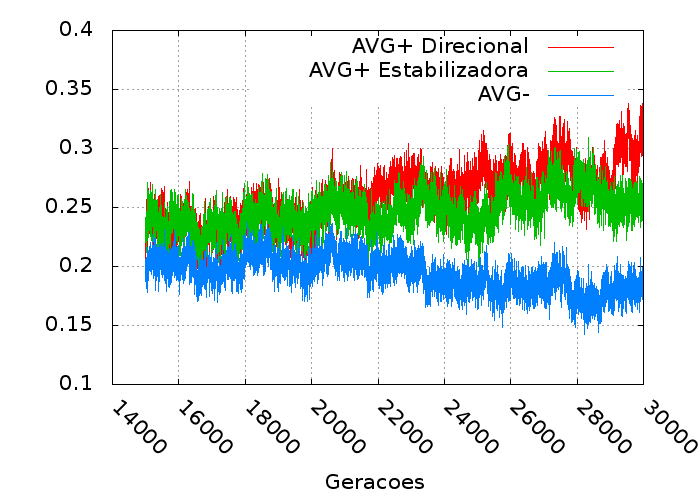
\includegraphics[width=70mm, height=50mm]{figuras/CoAVGPM90.png}}\vspace{11pt}
   \subfloat [$\Delta_S = 0.11$]{\label{CoAVG:Igual}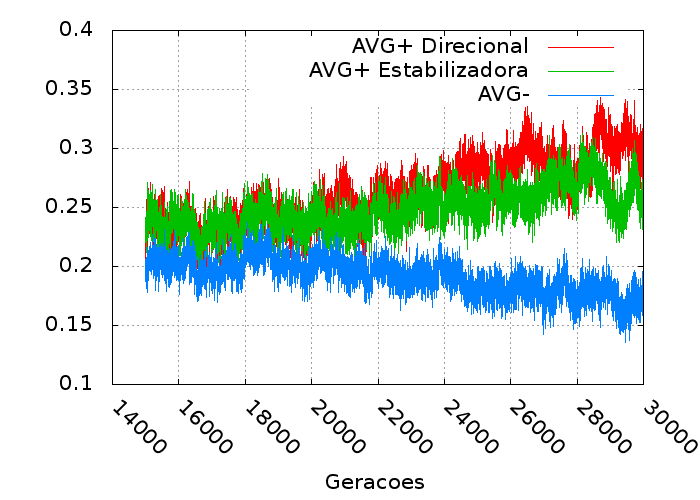
\includegraphics[width=70mm, height=50mm]{figuras/CoAVGPM110.png}}\\
   \vspace{-18pt}
   \subfloat [$\Delta_S = 0.18$]{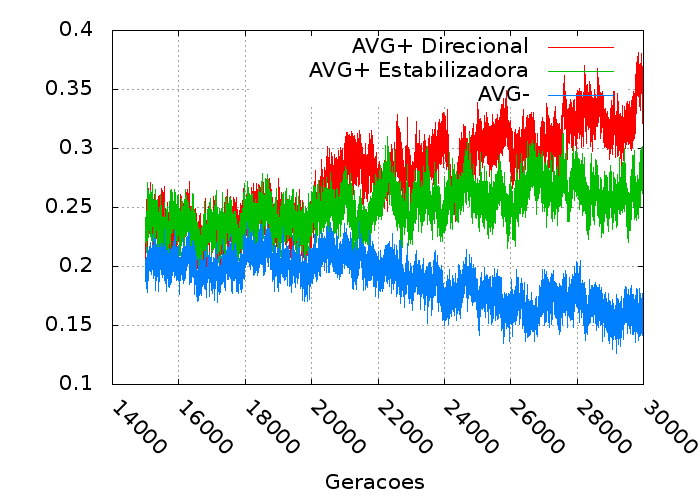
\includegraphics[width=70mm, height=50mm]{figuras/CoAVGPM180.png}}\vspace{11pt}
   \subfloat [$\Delta_S = 0.20$]{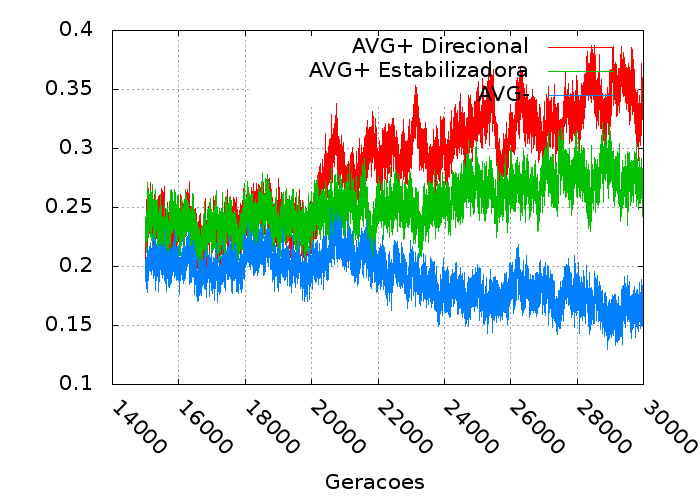
\includegraphics[width=70mm, height=50mm]{figuras/CoAVGPM200.png}}\\
   \caption{ Evolução da média das correlações dentro de cada módulo
      e entre módulos de uma população sofrendo seleção estabilizadora
      correlacionada com 2 módulos e seleção direcional em apenas um dos
   módulos, com diferentes valores de $\Delta_S$. $\mu/\mu_B = 5$, $Ne =
   5.000$, $m/p=5$. Seleção direcional a partir da geração $20.000$.}
   \label{CoAVG}
\end{figure}

